\documentclass[12pt]{article}

\usepackage{amssymb,amsmath,amsfonts,eurosym,geometry,ulem,graphicx,caption,color,setspace,sectsty,comment,footmisc,caption,natbib,pdflscape,subfigure,array,hyperref}

\normalem

\onehalfspacing
\newtheorem{theorem}{Theorem}
\newtheorem{corollary}[theorem]{Corollary}
\newtheorem{proposition}{Proposition}
\newenvironment{proof}[1][Proof]{\noindent\textbf{#1.} }{\ \rule{0.5em}{0.5em}}

\newtheorem{hyp}{Hypothesis}
\newtheorem{subhyp}{Hypothesis}[hyp]
\renewcommand{\thesubhyp}{\thehyp\alph{subhyp}}

\newcommand{\red}[1]{{\color{red} #1}}
\newcommand{\blue}[1]{{\color{blue} #1}}

\newcolumntype{L}[1]{>{\raggedright\let\newline\\arraybackslash\hspace{0pt}}m{#1}}
\newcolumntype{C}[1]{>{\centering\let\newline\\arraybackslash\hspace{0pt}}m{#1}}
\newcolumntype{R}[1]{>{\raggedleft\let\newline\\arraybackslash\hspace{0pt}}m{#1}}

\geometry{left=1.0in,right=1.0in,top=1.0in,bottom=1.0in}

\begin{document}




\begin{titlepage}
\title{Empirical Evidence on Stablecoins Peg Deviation\thanks{The usual disclaimer applies. All errors are ours.}}
\author{Michael Brooks \and Huachen Li}
\date{\today \\ DRAFT}


\maketitle
\begin{abstract}
\noindent This white paper documents empirical evidence on the effect of fluctuations of stablecoin peg deviation on the cryptocurrency market. Using daily data on Tether and EOSDT, we show shocks to Ethereum average transaction fee, Bitcoin price, and transaction volume are responsible and important to the peg deviation. Exogenous events, such as the COVID recession or bull-bear market cycles, significantly impact the stability both stablecoins but Tether price has an otherwise lower volatility than that of EOSDT.\\
\vspace{0in}\\
\noindent\textbf{Keywords:} Stablecoin, Tether, EOSDT, Structural Vector Autoregression\\
%\vspace{0in}\\
%\noindent\textbf{JEL Codes:} key1, key2, key3\\

\bigskip
\end{abstract}
\setcounter{page}{0}
\thispagestyle{empty}
\end{titlepage}
\pagebreak \newpage




\doublespacing


\section{Introduction}
Fiat-pegged cryptocurrencies, or stablecoins, combine the crypto advantage of privacy of payments and the fiat advantage of low price volatility. Stablecoins often achieve price stability through fiat- or crypto-collateralization. In contrast to traditional fixed currency regimes where the domestic central bank commits to expand or contract domestic money supply to maintain the peg, stablecoins rely on arbitrage from the demand side as a stabilization mechanism. Hence, real time stablecoin price of, say, USD, often experiences (sometimes sizable) fluctuations around the peg target. 

This paper studies the peg deviation of two stablecoins - Tether (USDT) and EOSDT. As a fiat-pegged, low volatility currency that operates on blockchains, USDT has become a popular vehicle among crypto traders.\footnote{According to CoinMarketCap.com, Tether is the second largest cryptocurrency by volume, the third largest by market cap, and the largest stablecoin by all metrics in July 2020. Since USDT is not commonly used as a medium of exchange for real goods and/or services, institutional and individual investors primarily hold USDT for cryptocurrency transacting or liquidity trading pairs.} Tether is issued by Tether Limited. Tether Limited collateralizes each Tether issuance with 1 USD and guarantees a one-to-one exchange. Thus, if the market price of USDT deviates from the peg, arbitragers are able to profit by exploiting the differences between the market price and the guaranteed exchange. 

EOSDT is a crypto-backed stablecoin that also aims to peg to the USD at an one-to-one rate. The main differentiator is that EOSDT is based on a cross-chain decentralized finance (DeFi) ecosystem called Equilibrium. The Equilibrium protocol allows smart contracts that collateralize individual investor's crypto holding free of custodial risk. Further, EOSDT serves as a great comparison to Tether because the EOS blockchain that Equilibrium uses is faster and provides more versatile infrastructure for smart contracts. 

Since USDT and EOSDT both rely on collateralization and the demand effect of arbitrage to maintain the peg, we study the effects of average Ethereum block fees, Bitcoin (BTC) price, and trading volume on peg deviation using a structural vector autoregression (SVAR) model. Further, differences in the underlying blockchain ecosystem allow us to compare and evaluate the stability of USDT and EOSDT. To this front, we extend the SVAR to allow time-varying parameters (TVP) and stochastic volatility (SV) to account for recent events such as the COVID-19 recession and the crypto black Thursday. We adopt Bayesian techniques to estimate the SVAR following \cite{primiceri} and \cite{cfp}. The algorithm relies on a Gibbs sampler from a Markov Chain Monte Carlo (MCMC) routine that estimates the TVP-SV-SVAR block by block. 

The results of this paper are threefold. First, we find significant changes in stability of the stablecoin prices during the COVID recession according the SV analysis. Second, shocks to Ethereum average transaction fees, Bitcoin prices, and Tether and EOSDT trading volume affect the peg deviation. Third, these effects appear to be dependent on not only the COVID recession but also bull-bear market cycles.

This paper is related to the literature on cryptocurrency. While the majority of this literature is devoted to Bitcoin, a few papers study the role of stablecoins such as Tether. For example, \cite{lyons} document the arbitrage mechanism behind USDT trading and show its importance in stabilizing the market prices around peg. The authors use a rolling window estimate of BTC volatility to show USDT can have a premium up to 100 basis points during the COVID-19 recession. This paper is also close to \cite{wei} who examines the relationship between USDT grants and BTC returns using a VAR model. The author finds reduced-form evidence that USDT issuance does not affect BTC prices but may positively affect BTC daily volume. 

We discuss data of the analysis in Section 2. Section 3 describes the SVAR model and estimation methods. Section 4 includes the results about stochastic volatility and impulse response functions. Chapter 5 concludes. 





\section{Motivation and Data}
This section describes the data and motivating observations that warrant a structural analysis. First, we focus on the price movements of USDT and EOSDT. Because the peg target of both USDT and EOSDT is one U.S. Dollar, we define peg deviation, $x_t$, as when the stablecoin price fluctuates away from the peg target. Specifically, let $p_t$ denote the daily closing price of USDT or EOSDT $x_t \equiv p_t - 1$.\footnote{Daily closing price is the price of USDT or EOSDT at 11:59PM of the day. Since both stablecoins trade continuously, the closing price is an arbitrary snapshot of the price.} 

\begin{figure}
  \centering
  \caption{USDT and EOSDT Peg Deviation}
  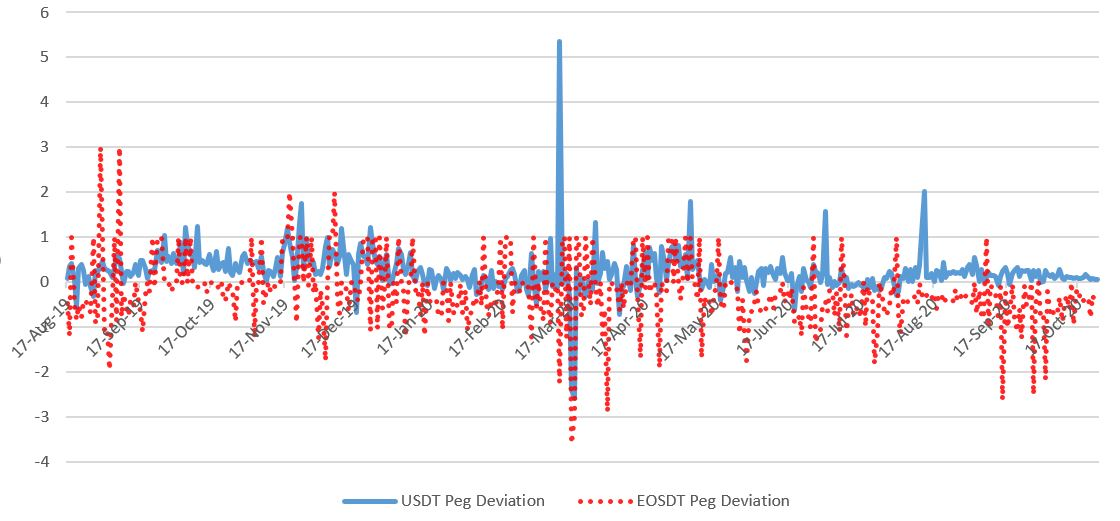
\includegraphics[width=1\textwidth]{pegdeviationplot}
  \label{pegdevplot}
\end{figure}


Figure \ref{pegdevplot} plots peg deviations for USDT (in solid blue line) and EOSDT (in solid read line) from August 17, 2019 to October 25, 2020. To reiterate, a positive (negative) peg deviation implies the stablecoin is trading at a premium (discount) over the U.S. Dollar. A visual inspection shows small correlation between the USDT and EOSDT series. In many cases, counter-cyclicality is observed, implying fundamental differences exist in how USDT and EOSDT prices deviate from the peg target. 


\begin{table}
		\caption {Summary Statistics}\label{tablestats}
		\begin{tabular}{ |p{5cm}||p{3cm}|p{3cm}|p{3cm}|  }
			\hline
			& Mean & Standard Deviation & $1^{\text{st}}$ order autocorrelation\\
			\hline
			USDT Peg Deviation (\%) &  0.24    & 0.46 &  0.15\\
			EOSDT Peg Deviation(\%) & -0.23    & 0.74 &  0.09\\
			Ethereum Avg. Fee (ETH)  &  0.003    & 0.004 &  0.79\\
			USDT Daily Volume (\$)  &  3.46e10   & 1.59e10 &  0.79\\
			EOSDT Daily Volume (\$)	&  5.70e5   & 2.04e6 &  0.85\\
			BTC Price (\$)     		&  8545.76    & 1247.99 &  0.95\\
			\hline
		\end{tabular}

{\raggedright \small Notes: Sample size is August 17, 2019 to October 25, 2020. Sample correlation between USDT and EOSDT peg deviation is 0.23. \par}	
\end{table}



Table \ref{tablestats} displays the summary statistics of the USDT and EOSDT peg deviation. The unconditional first moment implies on average USDT has been trading at a premium, whereas EOSDT has been trading at a discount to the U.S Dollar within the sample. Furthermore, EOSDT peg deviation is more volatile despite the large outlier in USDT peg deviation around black Thursday. In other words, the USDT peg appears to be more stable that that of EOSDT at least unconditionally. The correlation and first order auto-correlation are low for both series. 

Given the observation that large differences in the mean and standard deviation of USDT and EOSDT peg deviation exist, a natural questions is how do the two stablecoins respond to changes in other cryptocurrency fundamentals, namely daily transaction volume of the two stablecoins, BTC price, and Ethereum average transaction fee. Table \ref{tablestats} also reports the summary statistics on these metrics. 

A few additional observation about Table \ref{tablestats} are worth noting. First, aside of support the dominance of USDT as a stablecoin, USDT daily volume has a much higher degree of auto-correlation than that of EOSDT. Second, BTC price also exhibits a high first order auto-correlation. Thus, it is likely that USDT volume inherits this property from BTC price. As mentioned earlier, one of the primary purposes to hold USDT is for transactions of other cryptocurrencies. Third, Ethereum average transaction fee is a measure of average fee when a transaction is processed and confirmed by a miner. Since there is a limited number of spots for each block and investors expecting to have the transaction order fulfilled need to bid for the spots, a spike in average transaction fee may indicate a congestion in the network. This is especially true for arbitrage traders because fulfillment of order is a matter of profits. Thus, arbitrageurs have the incentive to bid up the transaction costs. Note that the average transaction fee also displays a high degree of first order autocorrelation.



\section{Econometric Methodology}
This section outlines the TVP-SV-SVAR model and identification strategy. We describe the Bayesian methods to estimate the time-varying parameters and stochastic volatility following \cite{primiceri} and \cite{cfp}. 

\subsection{Structural Vector Autoregression}
Let $y_t = [f_t, \Delta{P_t}, x_t, \Delta{V_t}]$ the $4\times1$ vector of endogenous variables of sample size $n$ where $f_t$, $P_t$, $x_t$, $V_t$, and $\Delta$ denote average Ethereum transaction fees, natural log of BTC price, USDT (EOSDT) peg deviation, natural log of USDT (EOSDT) volume, and the first difference operator. The $p^{th}$ order SVAR can be written as
\begin{equation}\label{svar}
y_t = B_{0,t}c_t + B_{1,t}y_{t-1} + ... + B_{p,t}y_{t-p} + A_t^{-1}\Sigma_t\epsilon_t, \,\,\,\,\, \epsilon_t\sim{N}(0,I),
\end{equation}
where $B_{i,t}$ are $n\times{n}$ time-varying regression coefficients, $c_t$ is the $4\times1$ time-varying constants, $A_t$ is the time-varying contemporaneous matrix, $\Sigma_t = diag(\sigma_{m,t})$ is a diagonal matrix that contains the stochastic volatility (time-varying standard deviations) of the structural shocks $\epsilon_t$. Equation \eqref{svar} can be written in the companion form of 
\begin{equation}
y_t = X_t'B_t + A_t^{-1}\Sigma_t\epsilon_t,
\end{equation}
where $X_t\equiv{I}\otimes[c_t', y_{t-1}', ... , y_{t-p}']$ and $B_t\equiv[vec(B_{i,t}')]$ for $i=1,... ,p$. 
Following conventions in the TVP-SV-SVAR literature, we assume the TVPs and SVs evolve as (geometric) random walks:
\begin{equation}
a_t = a_{t-1} + u_t;
\end{equation}
\begin{equation}
B_t = B_{t-1} + v_t;
\end{equation}
\begin{equation}
log\sigma_{m,t} = log\sigma_{m,t-1} + \eta_t,
\end{equation}
where $u_t$, $v_t$, and $\eta_t$ are independent, mean zero error terms of the random walk evolutions of the TVPs and SVs. Let $\mathcal{V}$ be the variance covariance matrix of the error terms,
\begin{equation}
\mathcal{V} = var(\begin{bmatrix}
\epsilon_t \\ v_t \\ u_t \\ \eta_t\\
\end{bmatrix})
=
 \begin{bmatrix}
I_n & 0 & 0 & 0\\
0   & V & 0 & 0 \\
0   & 0 & Q & 0\\
0   & 0 & 0 & W\\
\end{bmatrix}. 
\end{equation}


\subsection{Estimation}
Estimation of the model relies on a Bayesian MCMC routine that produces posterior estimates of the TVPs $a_t$ and $B_t$ and the SVs $\sigma_{m,t}$. We follow the \cite{cfp} algorithm and briefly describe the general steps below. 

\begin{itemize}
	\item[1] Initialize $A^0$, $B^0$, $\Sigma^0$, $\mathcal{V}^0$, and $s^0$ and set draw counter $i=1$.\footnote{$s$ is an auxiliary variable for sampling the SVs.}
	\item[2] Draw $B^i$ from $p[B|y^T, A^{i-1}, \Sigma^{i-1}, \mathcal{V}^{i-1}, s^{i-1}]I_B(B^i)$ where $I_B(B^i)$ is a truncation function that ensures the stationarity of the $B^i$ draws. 
	\item[3] Draw $A^i$ from $p[A|y^T, B^i, \Sigma^{i-1}, \mathcal{V}^{i-1}, s^{i-1}]$. 
	\item[4] Draw $\Sigma^i$ and $s^i$ following \cite{kim}.
	\item[5] Draw $\mathcal{V}^i$ from $p[A|y^T, A^{i}, B^i, \Sigma^{i}, s^{i}]$.
	\item[6] Repeat steps 2-5 for $K$ times.
\end{itemize}

In practice, we set the lag order $p=2$ as optimally chosen by AIC, BIC and SQIC, the number of draws $K = 60000$ with a burn-in of $40000$ draws. For the remaining $20000$ draws, a thinning factor of $40$ is applied, resulting in $500$ posterior draws. The acceptance rates of the $A_t$ draws and the $B_t$ draws are 35\% and 65\%. 

 We assume the contemporaneous impact matrix $A_t$ is a lower triangular matrix where the diagonal entries are ones. In other words, the model is exactly identified at impact. The structural model is written as
 \begin{equation}
 y_t = X_t'B_t +
  \begin{bmatrix}
 1   & 0 & 0 & 0\\
 a_{21,t}   & 1 & 0 & 0 \\
 a_{31,t}   & a_{32,t} & 1 & 0\\
 a_{41,t}   & a_{42,t} & a_{43,t} & 1\\
 \end{bmatrix}
  \begin{bmatrix}
 \Sigma_{1,t} & 0 & 0 & 0\\
 0   & \Sigma_{2,t} & 0 & 0 \\
 0   & 0 & \Sigma_{3,t} & 0\\
 0   & 0 & 0 & \Sigma_{4,t}\\
 \end{bmatrix}
 \begin{bmatrix}
 \epsilon_t^f \\ \epsilon_t^P \\ \epsilon_t^x \\ \epsilon_t^V\\
 \end{bmatrix}
 \end{equation}
 
 
 Two TVP-SV-SVARs are estimated using USDT and EOSDT peg deviation and their volume, respectively. These SVARs are estimated with daily data. The first 90 observations are used as a training sample to setup the priors. We assume proper conjugate priors for $a$, $B$, $V$, $Q$, $W$, and $\Sigma$. Specifically, the prior mean and variance on $a$ and $\Sigma$ are estimated from the training sample using maximum likelihood methods and $B$ using OLS. 



\section{Empirical Results}
\subsection{Stochastic Volatility}
We first report the SV ($\sigma_{m,t}$) of each structural shock in blue and their 95\% posterior tunnels in red in Figure \ref{sv}. Several findings are noteworthy which we outline below.

\begin{center}
[Figure \ref{sv} about here.]
\end{center}



First, the estimated SV of Ethereum average transaction fee stays relatively stable until around April 2020 which is well into the COVID-19 recession. Large fluctuations appear to lag the initial COVID shock (black Thursday) by at least one month. This indicates that average transaction fee is low volatility outside of significant shocks to the economy. 

Second, the SV of Bitcoin price shows a significant spike on black Thursday. However, we also observe a noticeable degree of fluctuations across the entire sample that are statistically significant according to the 95\% error bands. This result reinforces the common prior that Bitcoin price is volatile and the impact of an exogenous shock, i.e. the COVID recession, is large on the volatility of Bitcoin price.

Third, the SVs of USDT and EOSDT peg deviations show different implications about the stability of the two stablecoins. The SV of USDT from the beginning of the sample till the black Thursday has been consistently declining. This suggests the stability of USDT has been improving. Disrupted by the COVID shock, the SV of USDT spikes in a similar fashion to that of Bitcoin. The spike quickly diminishes and the SV of USDT resumes to a similar downward trend. These observations indicate USDT's stability has been steadily improving despite of the COVID shocks. 

On the other hand, the SV of EOSDT peg deviation exhibits large movements that are statistically significant over the entire sample. The black Thursday spike is visible but does not show a comparable magnitude to that of Bitcoin and USDT. These results suggest EOSDT is less stable on average (compare to USDT) but is also less responsive to large exogenous shocks. 

Lastly, the median estimates of the USDT volume appear to have a positive drift while that of the EOSDT volume declines over time. However, these SVs display minimal statistically significant fluctuations across the entire sample. This suggests large spikes in cryptocurrency prices and economic recession do not have a large impact the stability of the trading volume. 



\subsection{Impulse Response Functions}
We evaluate the transmission mechanism of the structural shocks in the section. The analysis focuses on how the peg deviations of USDT and EOSDT respond to the three structural shocks: Ethereum transaction fees shock, Bitcoin shock, and volume shock. Three dimension IRFs are reported to study whether or not time variations of the structural parameters play a role. Similar to \cite{cfp}, the size of the structural shocks are normalized to one across the sample so the time variations, if any, in the IRFs represent the shock propagation rather than the size of the shocks. 


\begin{center}
	[Figure \ref{shock13} about here.]
\end{center}

Figure \ref{shock13} plots the response of USDT (upper panel) and EOSDT (lower panel) peg deviation with respect to a positive one standard deviation shock to average Ethereum transaction fees. As expected, within 1-5 days, USDT prices deviate negatively by up to 20 basis points during the wake of the COVID recession. However, these responses display a sign change in July 2020. Specifically, the transaction fee shock could lead to a 10 basis point premium in USDT in the second half of the sample.


In contrary, EOSDT collects fees on the EOS network but we still observe a negative short term response of EOSDT price to a Ethereum transaction fee shock. In other words, there is no substitution effect among networks. EOSDT peg deviation reverts back to a negative short term response towards the end of the sample. 

These results indicate that an increase in average transaction fees adversely affect stablecoins peg deviation in the short term for the majority of the sample regardless of the network. This effect may be explained as investors treat transaction fees as an additional cost to hold stablecoins. It is worth noting that the effect of the transaction fee shock is transitory and the peg deviation for both stablecoins revert back to zero after around 10 days post shock. 

Additionally, the stablecoin boom in October 2020 appears to have different effects on Tether versus EOSDT. As the beginning of a new bull cycle, Tether begins to respond positively and persistently to a transaction fee shock. On the other hand, EOSDT displays a large trough response up to 25 basis points in October and the late sample. Thus, we believe market cycles are responsible for the contrast between the early sample (bear cycle) and late sample (bull cycle) responses. 


\begin{center}
	[Figure \ref{shock23} about here.]
\end{center}


Figure \ref{shock23} plots the response of USDT (upper panel) and EOSDT (lower panel) peg deviation with respect to a positive one standard deviation shock to Bitcoin prices. Immediately following a Bitcoin price shock, USDT exhibits a price premium in the first half of the sample till May 2020. This downward drift in the response is not observed in the EOSDT panel. An increase in Bitcoin price almost always leads to a negative peg deviation in EOSDT across the entire sample. This negative effect is around 5 basis points. 

Several interesting results are worth noting. First, a Bitcoin price shock affects USDT only by 1-2 basis points throughout the sample. As discussed, this effect is much larger for EOSDT. This may speak about the different levels of stability between the two stablecoins. Second, the Bitcoin price shock has transitory effects on the peg deviation of USDT and EOSDT within around two weeks before the peg deviation restores back to pre-shock level. Furthermore, during the early sample bear cycle, the difference in the USDT and EOSDT response to the same Bitcoin price shock suggests potential arbitrage opportunities between the two stablecoins, assuming efficient exchange market and trivial transaction costs. The potential arbitrage profit can be up to 6 basis points in early January and March of 2020.


\begin{center}
	[Figure \ref{shock43} about here.]
\end{center}


Figure \ref{shock43} plots the response of USDT (upper panel) and EOSDT (lower panel) peg deviation with respect to a positive one standard deviation shock to their own volume. An volume shock generates an oscillating short term response in the peg deviation of both stablecoins. These responses decrease within the first two days post shock before increase within the week. Thus, long term mean reversion is observed in both impulse responses of USDT and EOSDT.


Although the aggregate effect of the volume shock on the peg deviations is around zero, Figure \ref{shock43} is suggesting a similar implication that USDT appears to fluctuate to a smaller degree than EOSDT. For example, the USDT peg deviates by plus or minus 2 basis points facing an own volume shock. The EOSDT peg, on the other hand, can deviate by up to 6 basis points in either direction. This reinforces the findings in Figure 4 that USDT exhibits a higher degree of stability facing an external shock. 


\begin{center}
	[Figure \ref{shock32} about here.]
\end{center}


Next, we examine how a shock to the peg deviation in either Tether or EOSDT affect Bitcoin price. Figure \ref{shock32} plots the three dimensional IRF of bitcoin price with respect to a peg deviation shock with USDT in the upper panel and EOSDT in the lower panel. When the stablecoins are trading at a premium over their peg target, Bitcoin price can decrease by 15 basis points over the sample and the effect appears to last at least 30 days post shock. There is small time variation over the sample, indicating this negative effect is not dependent on the state of the market. Economically, a positive peg deviation is equivalent to an increased cost of stablecoin transaction. Holding everything else constant,  since many investors hold stablecoins as a medium of exchange to Bitcoin, an expensive stablecoin may disincentivize transactions thus lower the Bitcoin price. 


\begin{center}
	[Figure \ref{shock34} about here.]
\end{center}


Finally, we plot the three dimensional impulse responses of stablecoins own volume to a shock to their respective peg deviation in Figure \ref{shock34}. As shown in the upper panel, Tether volume decreases in the long-term by 5 basis points after the initial surge two days post shock. There is a small but visible downward drift in the long term effect across the sample. This indicates the Tether volume decline due to its higher price worsens over the sample. This is also evidence that law of demand appears to have persistent effect in the Tether market. 

The lower panel of Figure \ref{shock34} displays how EOSDT responds to its peg deviation shock. Immediately after impact, EOSDT volume decreases up to 4 basis points and converges to a long-run steady state of between 2 to 5 basis points throughout the sample. Large time variation, especially for horizons over 10 days post shock, is observed. Particularly during the beginning of the bull cycle in October, EOSDT volume exhibits the lowest long term response to its peg deviation shock. On contrary, during the peak of the bear cycle in April 2020, the long term EOSDT volume declines only by around 2 basis points. This indicates that EOSDT volume fluctuations are more likely to be dependent on the market cycle swings. Overall, the law of demand effect is still on full exhibition for EOSDT.


\section{Concluding Remarks}
In this paper, we use Bayesian SVAR models with time-varying parameters and stochastic volatility to examine the mechanism in which the fiat peg prices of Tether and EODST fluctuate. It is important to understand stablecoin peg deviations because stablecoin prices are designed to be maintained by demand. Thus, understanding fluctuations in the peg deviation can shed light on how stablecoins are perceived by the investors.

This paper documents three main results. First, Tether has a higher degree of stability over the sample but exogenous events such as the black Thursday can have a large effect on its stability. Second, an increase in Bitcoin price causes both stablecoins to trade at a discount in the short term but Tether and EOSDT prices respond to an increase in their own trading volume oppositely. Third, time-varying analysis suggests these results are dependent on the market cycle and exogenous events such as the bull-bear cycles and COVID recession.

Stablecoin prices can deviate from their peg often. Results of this paper provide a platform to analyze the determinants of stablecoin price fluctuations. Because of their dependence on arbitrage from investors to maintain the peg, prices of fiat collateralized stablecoins are susceptible to the state of the cryptocurrency market. 




\clearpage

\begin{figure}
	\centering
	\caption{USDT and EOSDT Peg Deviation}
	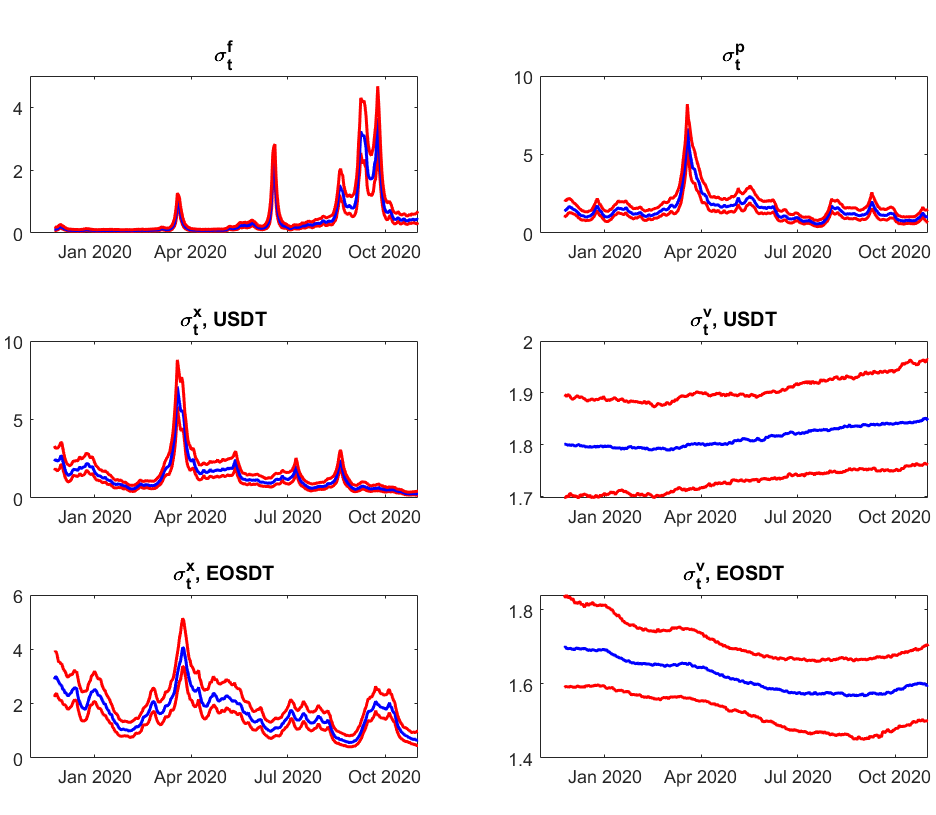
\includegraphics[width=1\textwidth]{SV}
	\label{sv}
		\begin{minipage}{1\textwidth} % choose width suitably
		{\footnotesize Notes: Blue line is the median estimate. Red lines are the 95\% posterior tunnels. X-axis: sample dates. Y-axis: magnitude of SV.\par}
	\end{minipage}
\end{figure}



\begin{figure}
	\centering
	\caption{Impulse Response of Peg Deviation to Average Transaction Fees Shock}
	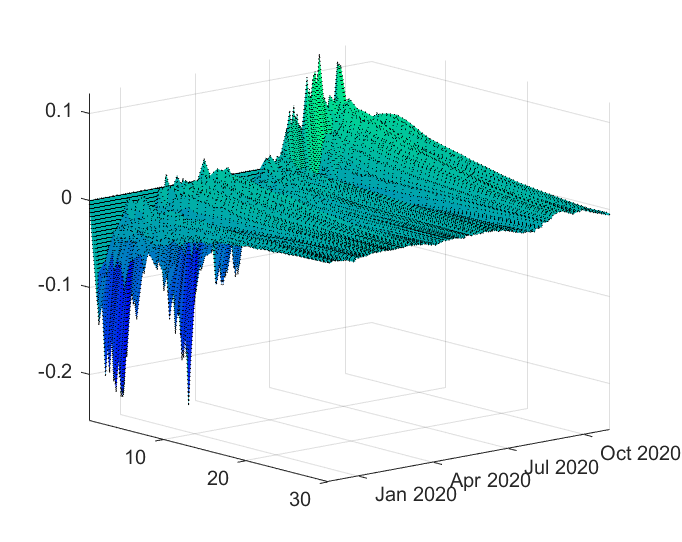
\includegraphics[width=0.7\textwidth]{shock1resp3}
	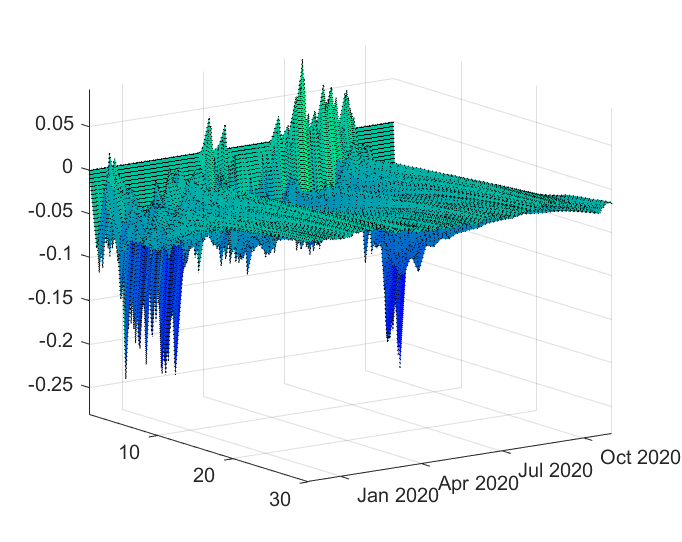
\includegraphics[width=0.7\textwidth]{shock1resp3eos}
	\label{shock13}
	\begin{minipage}{1\textwidth} % choose width suitably
		{\footnotesize Notes: Upper panel is USDT. Lower panel is EOSDT. X-axis: forecast horizons. Y-axis: magnitude of responses. Z-axis: sample dates. \par}
	\end{minipage}
\end{figure}


\begin{figure}
	\centering
	\caption{Impulse Response of Peg Deviation to BTC Price Shock}
	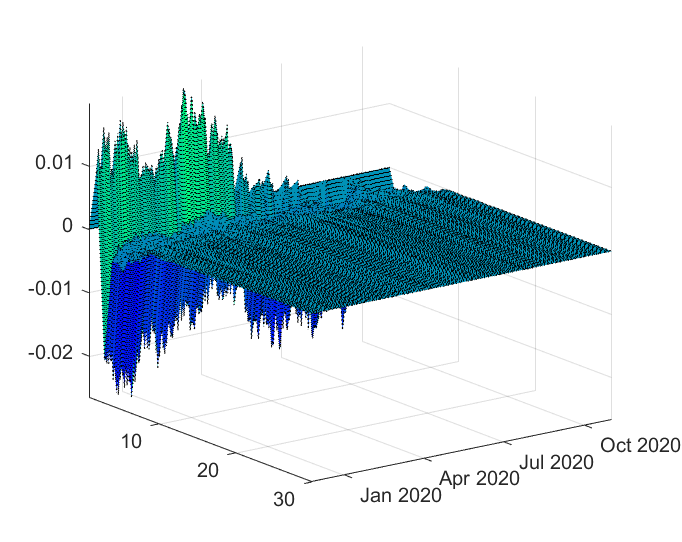
\includegraphics[width=0.7\textwidth]{shock2resp3}
	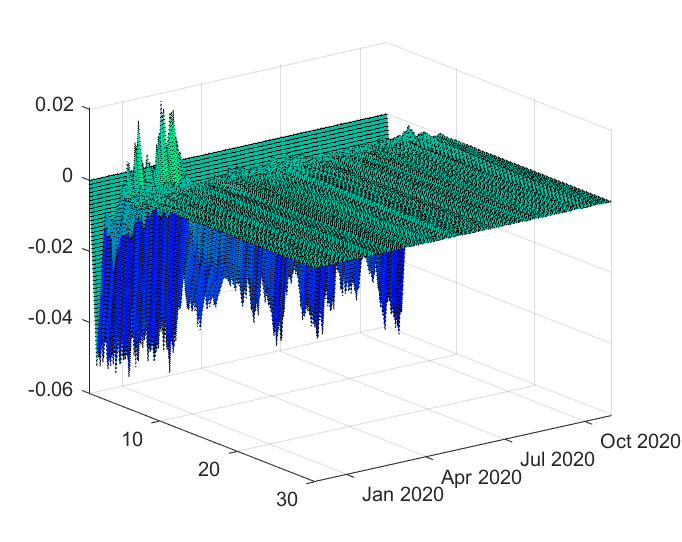
\includegraphics[width=0.7\textwidth]{shock2resp3eos}
	\label{shock23}
	\begin{minipage}{1\textwidth} 
		{\footnotesize Notes: Upper panel is USDT. Lower panel is EOSDT. X-axis: forecast horizons. Y-axis: magnitude of responses. Z-axis: sample dates. \par}
	\end{minipage}
\end{figure}

\begin{figure}
	\centering
	\caption{Impulse Response of Peg Deviation to Own Volume Shock}
	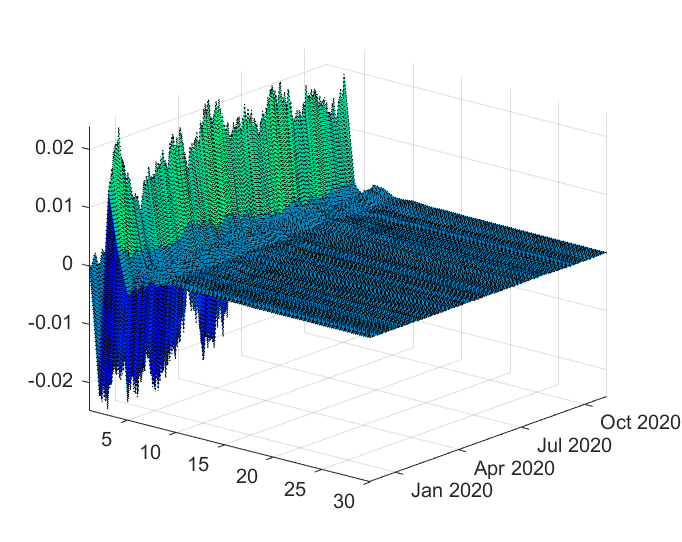
\includegraphics[width=0.7\textwidth]{shock4resp3}
	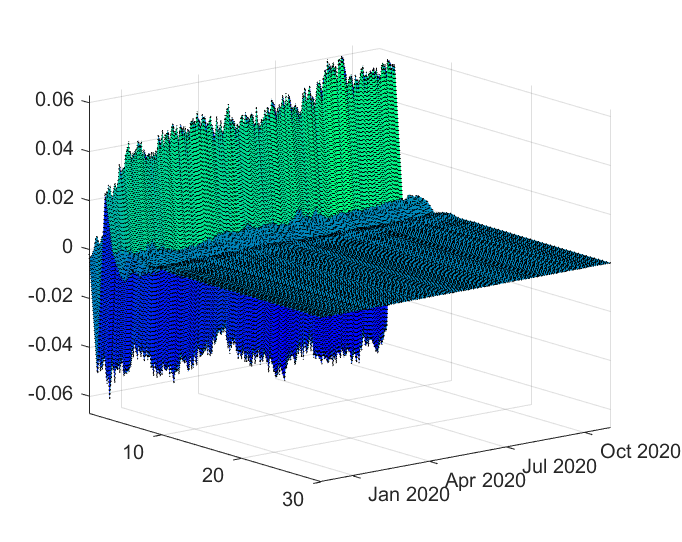
\includegraphics[width=0.7\textwidth]{shock4resp3eos}
	\label{shock43}
	\begin{minipage}{1\textwidth} 
		{\footnotesize Notes: Upper panel is USDT. Lower panel is EOSDT. X-axis: forecast horizons. Y-axis: magnitude of responses. Z-axis: sample dates. \par}
	\end{minipage}
\end{figure}


\begin{figure}
	\centering
	\caption{Impulse Response of Bitcoin Price to Peg Deviation Shock}
	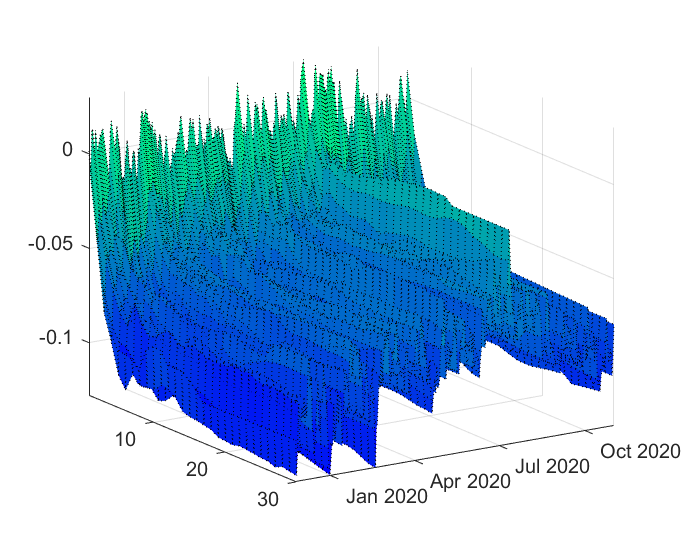
\includegraphics[width=0.7\textwidth]{shock3resp2cum}
	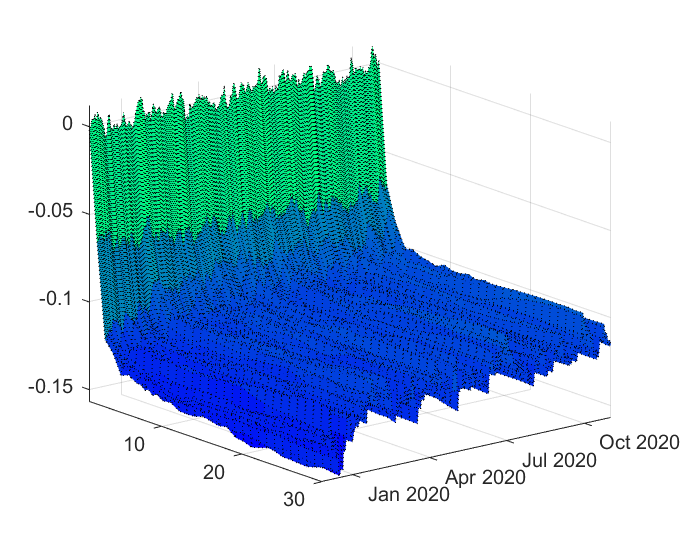
\includegraphics[width=0.7\textwidth]{shock3resp2cumeos}
	\label{shock32}
	\begin{minipage}{1\textwidth} 
		{\footnotesize Notes: Upper panel is USDT. Lower panel is EOSDT. X-axis: forecast horizons. Y-axis: magnitude of responses. Z-axis: sample dates. \par}
	\end{minipage}
\end{figure}

\begin{figure}
	\centering
	\caption{Impulse Response of Stablecoin Own Volume to Peg Deviation Shock}
	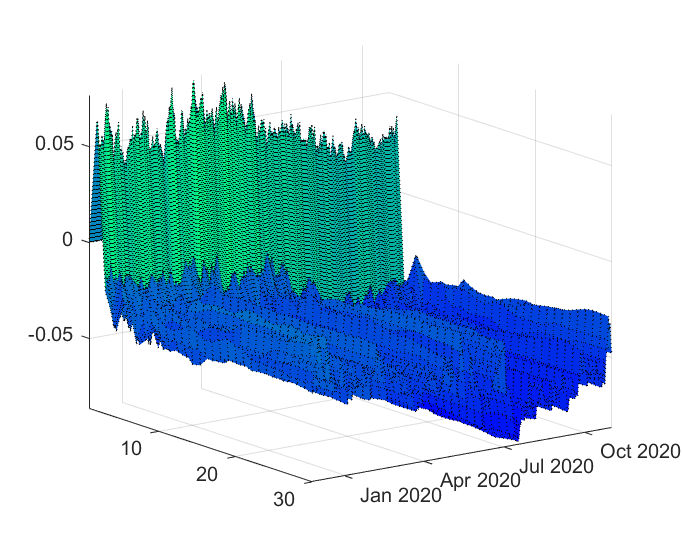
\includegraphics[width=0.7\textwidth]{shock3resp4cum}
	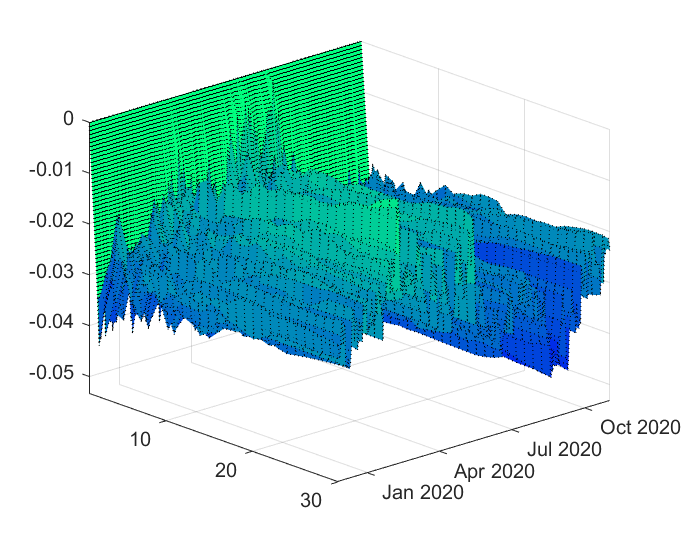
\includegraphics[width=0.7\textwidth]{shock3resp4cumeos}
	\label{shock34}
	\begin{minipage}{1\textwidth} 
		{\footnotesize Notes: Upper panel is USDT. Lower panel is EOSDT. X-axis: forecast horizons. Y-axis: magnitude of responses. Z-axis: sample dates. \par}
	\end{minipage}
\end{figure}


\clearpage
\singlespacing
\bibliographystyle{apa}
\bibliography{stablecoinbib}



\clearpage

\onehalfspacing




\end{document}